\documentclass[../../main.tex]{subfiles}

\graphicspath{{../../image/}{../../figure/}}

\begin{document}

\section{归约为场方程}\label{section:ch01-归约为场方程}

上述简化虽在许多应用中已足够，但对我们的目的而言限制过强：我们必须广泛处理熵类量的平衡律，这类量在 Lebesgue 测度为零的激波阵面上会产生非零生成。

初看起来，\cref{section:ch01-平衡律的表述} 中引入的平衡律概念似乎过于一般而无从使用。然而事实证明，平衡要求\cref{align:ch01-balance-primitive} 对密度通量函数施加了极强的限制。具体地说，$q_{\mathscr{D}}$ 在 $X\in\partial\mathscr{D}$ 处的值可能仅通过 $X$ 处的外法向 $N$ 而依赖于 $\mathscr{D}$，且这种依赖是“线性的”。这使平衡律相当具体，将其归约为一个场方程。

\begin{theorem}\label{theorem:ch01-场方程归约}
设 $\mathscr{X}$ 上的平衡律\cref{align:ch01-balance-primitive} 中，$\mathscr{P}$ 是带符号 Radon 测度，$\mathscr{Q}_{\mathscr{D}}$ 通过\cref{align:ch01-flux-density} 由密度通量函数 $q_{\mathscr{D}}$ 诱导，且对一切真域 $\mathscr{D}$ 与任意 $X\in\partial\mathscr{D}$，$|q_{\mathscr{D}}(X)|\leqslant C$。则：
\begin{enumerate}
\item\label{item:ch01-场方程归约-i} 对每个 $N\in\mathbb{S}^{k-1}$，伴随一个 $\mathscr{X}$ 上的有界可测函数 $a_{N}$，具有下述性质：设 $\mathscr{D}$ 为 $\mathscr{X}$ 中任一真域，$X$ 为 $\partial\mathscr{D}$ 上某一点，$\mathscr{D}$ 在该点的外单位法向量存在且等于 $N$。进一步假设 $X$ 是 $q_{\mathscr{D}}$ 关于 $\mathscr{H}^{k-1}$ 的 Lebesgue 点，且 $|\mathscr{P}|$ 在 $X$ 处关于 Lebesgue 测度的上导数有限。则
\begin{align}
q_{\mathscr{D}}(X)=a_{N}(X).\label{align:ch01-qd-aN}
\end{align}
\item\label{item:ch01-场方程归约-ii} 存在向量场 $A\in L^{\infty}\bigl(\mathscr{X};\mathbb{M}^{1\times k}\bigr)$，使得对任意固定的 $N\in\mathbb{S}^{k-1}$，
\begin{align}
a_{N}(X)=A(X)N,\qquad\text{a.e. 在 }\mathscr{X}\text{ 上}.\label{align:ch01-aN-AN}
\end{align}
\item\label{item:ch01-场方程归约-iii} 函数 $A$ 满足场方程
\begin{align}
\operatorname{div} A=\mathscr{P},\label{align:ch01-divA-P}
\end{align}
在 $\mathscr{X}$ 上分布意义下。
\end{enumerate}
\end{theorem}

\begin{proof}
固定任一 $N\in\mathbb{S}^{k-1}$，再取任一余维为 $1$、法向为 $N$ 且与 $\mathscr{X}$ 相交非空的超平面 $\mathscr{C}$。对 $X\in\mathscr{C}\cap\mathscr{X}$，记 $\mathscr{B}_{r}^{-}(X)$ 为半球 $\{Y\in\mathscr{B}_{r}(X):(Y-X)\cdot N<0\}$。极限
\begin{align}
a_{N}(X)=\lim_{r\downarrow 0}\frac{1}{\mathscr{H}^{k-1}\bigl(\mathscr{C}\cap\mathscr{B}_{r}(X)\bigr)}\int_{\mathscr{C}\cap\mathscr{B}_{r}(X)}q_{\mathscr{B}_{r}^{-}(X)}(Y)\,\mathrm{d}\mathscr{H}^{k-1}(Y),\label{align:ch01-aN-limit}
\end{align}
对 $\mathscr{H}^{k-1}$ 几乎所有 $X\in\mathscr{C}\cap\mathscr{X}$ 存在，并定义一个有界、$\mathscr{H}^{k-1}$-可测函数。对每个法向为 $N$ 的超平面重复上述构造，便在整个 $\mathscr{X}$ 上定义了 $a_{N}$。

为研究 $a_{N}$ 的性质，固定 $N\in\mathbb{S}^{k-1}$，连同法向为 $N$ 的超平面 $\mathscr{C}$，以及 $\mathscr{X}$ 中一个球 $\mathscr{B}$，其球心位于 $\mathscr{C}\cap\mathscr{X}$ 上某点。然后将平衡律应用于柱域
\begin{align}
\mathscr{D}=\bigcup_{-\delta<\tau<\varepsilon}\mathscr{A}_{\tau},\qquad
\mathscr{A}_{\tau}=\{X:X-\tau N\in\mathscr{C}\cap\mathscr{B}\},\label{align:ch01-cylinder}
\end{align}
其中 $\delta$ 与 $\varepsilon$ 为小的非负数。由此得到
\begin{align}
\int_{\mathscr{A}_{\varepsilon}}a_{N}(X)\,\mathrm{d}\mathscr{H}^{k-1}(X)+\int_{\mathscr{A}_{-\delta}}a_{-N}(X)\,\mathrm{d}\mathscr{H}^{k-1}(X)=\mathscr{P}(\mathscr{D})+O(\delta)+O(\varepsilon),\label{align:ch01-cylinder-balance}
\end{align}
其中 $O(\delta)$ 与 $O(\varepsilon)$ 两项给出柱域侧面上的通量贡献。令 $\delta=0$ 而令 $\varepsilon\downarrow 0$，从\cref{align:ch01-cylinder-balance} 导出一个估计；将其应用于一切球 $\mathscr{B}$，即得当 $\tau\downarrow 0$ 时，$a_{N}(X+\tau N)\to -a_{-N}(X)$，在 $L^{\infty}(\mathscr{C}\cap\mathscr{X})$ 中弱$^{*}$ 意义下。类似地，令 $\varepsilon=0$ 而令 $\delta\downarrow 0$，推得当 $\tau\uparrow 0$ 时，$a_{-N}(X+\tau N)\to -a_{N}(X)$，同样在 $L^{\infty}(\mathscr{C}\cap\mathscr{X})$ 中弱$^{*}$ 意义下。特别地，这蕴涵 $a_{N}$ 在 $\mathscr{X}$ 上 Lebesgue 可测。

回到\cref{align:ch01-cylinder-balance}，现在令 $\delta\downarrow 0$ 且 $\varepsilon\downarrow 0$，我们得到 $a_{-N}(X)=-a_{N}(X)$，对 $\mathscr{H}^{k-1}$ 几乎所有 $X\in\mathscr{C}\cap\mathscr{X}$ 成立，除非 $\mathscr{C}$ 属于那族（至多可数）法向为 $N$ 且 $|\mathscr{P}|(\mathscr{C}\cap\mathscr{X})>0$ 的超平面。此后将这些例外超平面称为\emph{奇异}的。

\begin{figure}[ht]
\centering
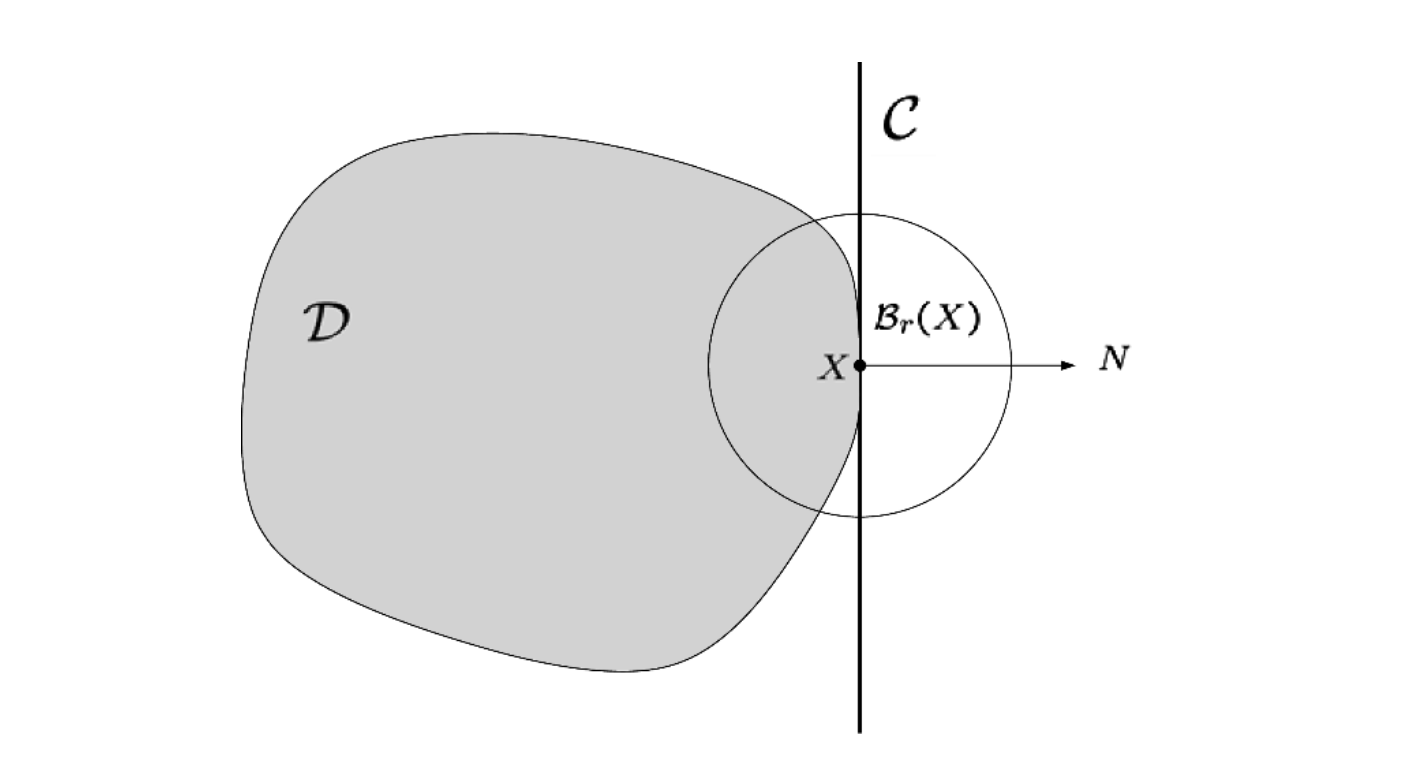
\includegraphics[width=0.72\textwidth]{../../image/ch01-fig02-01.png}
\caption{柱域论证：超平面 $\mathscr{C}$、外法向 $N$ 与半球 $\mathscr{B}_{r}(X)$。}\label{figure:ch01-cylinder-construction}
\end{figure}

为证明\cref{item:ch01-场方程归约-i}，考虑 $\mathscr{X}$ 中任一真域 $\mathscr{D}$，并固定 $X\in\partial\mathscr{D}$ 为外单位法向为 $N$、切超平面为 $\mathscr{C}$ 的点。进一步假设 $X$ 是 $q_{\mathscr{D}}$ 的 Lebesgue 点，且 $|\mathscr{P}|$ 在 $X$ 处关于 Lebesgue 测度的上导数有限。取正的小量 $r$，先对域 $\mathscr{D}\cap\mathscr{B}_{r}(X)$、再对半球 $\{Y\in\mathscr{B}_{r}(X):(Y-X)\cdot N<0\}$ 写出平衡律；见\cref{figure:ch01-cylinder-construction}。

将所得两式合并，得到
\begin{align}
\int_{\partial\mathscr{D}\cap\mathscr{B}_{r}(X)}q_{\mathscr{D}}(Y)\,\mathrm{d}\mathscr{H}^{k-1}(Y)-\int_{\mathscr{C}\cap\mathscr{B}_{r}(X)}a_{N}(Y)\,\mathrm{d}\mathscr{H}^{k-1}(Y)=o(r^{k-1}).\label{align:ch01-semiball-comparison}
\end{align}
以 $r^{k-1}$ 除\cref{align:ch01-semiball-comparison}，令 $r\downarrow 0$，并回忆\cref{align:ch01-aN-limit}，即得\cref{align:ch01-qd-aN}，从而证明了定理的第 (i) 断言。

\begin{figure}[ht]
\centering
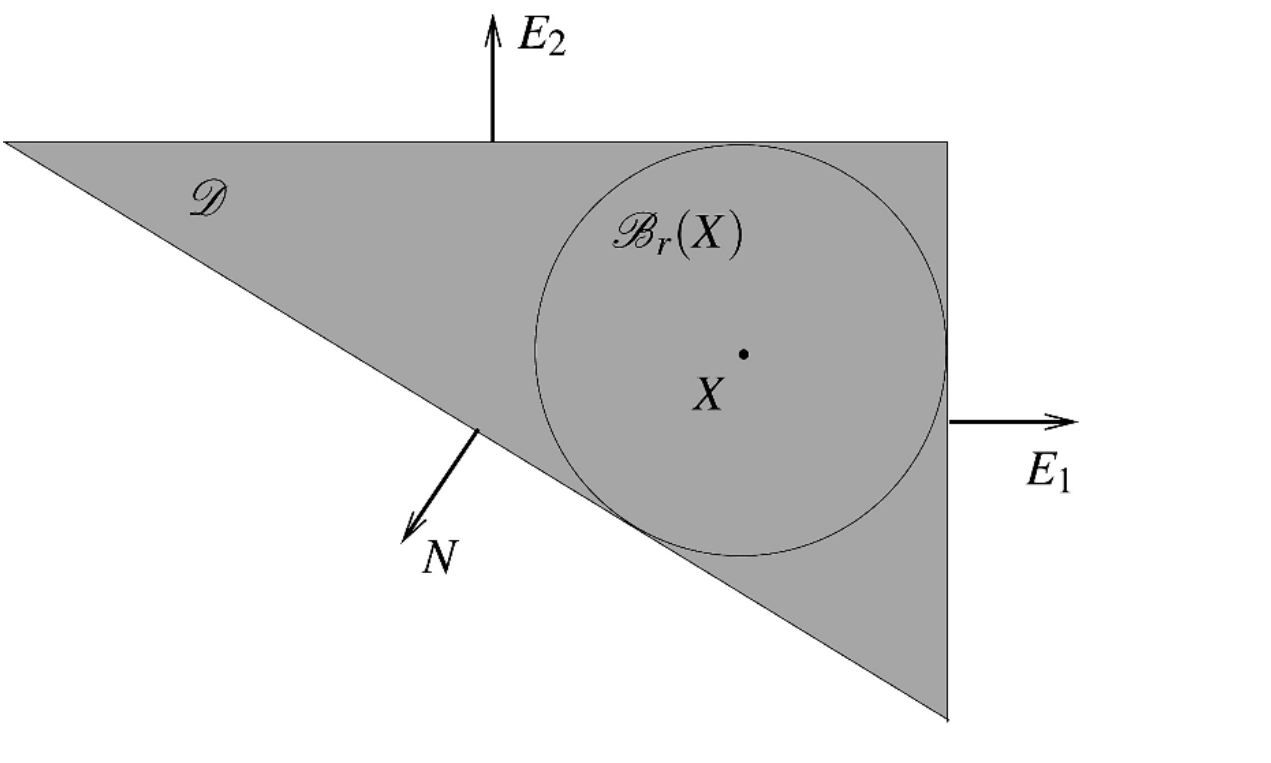
\includegraphics[width=0.72\textwidth]{../../image/ch01-fig02-02.png}
\caption{Cauchy 四面体论证在 $k=2$、$N_{1},N_{2}$ 均为负时的情形。}\label{figure:ch01-cauchy-tetrahedron}
\end{figure}

我们将借助著名的 Cauchy 四面体论证来验证\cref{item:ch01-场方程归约-ii}。在 $\mathbb{R}^{k}$ 中引入标准正交基 $\{E_{\alpha}:\alpha=1,\cdots,k\}$，并组装 $m$ 行向量场 $A\in L^{\infty}(\mathscr{X};\mathbb{M}^{1\times k})$，其分量为 $a_{E_{\alpha}}$：
\begin{align}
A(X)=\bigl[a_{E_{1}}(X),\cdots,a_{E_{k}}(X)\bigr].\label{align:ch01-A-components}
\end{align}
固定任一 $N\in\mathbb{S}^{k-1}$，其分量 $N_{\alpha}$ 非零（当某些 $N_{\alpha}$ 为零时论证需稍作修改），并取 $X\in\mathscr{X}$ 满足以下性质：$X$ 是 $k+1$ 个函数 $a_{E_{1}},\cdots,a_{E_{k}}$ 与 $a_{N}$ 的 Lebesgue 点；$|\mathscr{P}|$ 在 $X$ 处关于 Lebesgue 测度的上导数有限。取正的小量 $r$，考虑单纯形\footnote{Cauchy 四面体论证得名于 $k=3$ 的特殊情形。\cref{figure:ch01-cauchy-tetrahedron} 描绘了 $k=2$ 且 $N_{1},N_{2}$ 均为负时的设置。}
\begin{align}
\mathscr{D}=\{Y:(Y_{\alpha}-X_{\alpha})\operatorname{sgn}N_{\alpha}>-r,\ \alpha=1,\cdots,k;\ (Y-X)\cdot N<r\}.\label{align:ch01-simplex}
\end{align}
注意到 $\partial\mathscr{D}$ 由一个外法向为 $N$ 的面 $\mathscr{C}$ 与 $k$ 个面 $\mathscr{C}_{\alpha}$（$\alpha=1,\cdots,k$）组成，后者的外法向分别为 $(-\operatorname{sgn}N_{\alpha})E_{\alpha}$。此外有 $\mathscr{H}^{k-1}(\mathscr{C}_{\alpha})=|N_{\alpha}|\mathscr{H}^{k-1}(\mathscr{C})$。选取 $r$ 使 $\mathscr{D}$ 的任何一面都不落在奇异超平面上。于是 $\mathscr{D}$ 的平衡律写为
\begin{align}
\int_{\mathscr{C}}a_{N}\,\mathrm{d}\mathscr{H}^{k-1}-\sum_{\alpha=1}^{k}(\operatorname{sgn}N_{\alpha})\int_{\mathscr{C}_{\alpha}}a_{E_{\alpha}}\,\mathrm{d}\mathscr{H}^{k-1}=\mathscr{P}(\mathscr{D}).\label{align:ch01-simplex-balance}
\end{align}
以 $\mathscr{H}^{k-1}(\mathscr{C})$ 除\cref{align:ch01-simplex-balance}，再沿任一趋于零且避开（至多可数个）使 $\mathscr{D}$ 某面落在奇异超平面上的 $r$ 值序列取极限，得到
\begin{align}
a_{N}(X)=\sum_{\alpha=1}^{k}a_{E_{\alpha}}(X)N_{\alpha}=A(X)N,\label{align:ch01-aN-sum}
\end{align}
这就证明了\cref{align:ch01-aN-AN}。

还须证明\cref{item:ch01-场方程归约-iii}。当 $A$ Lipschitz 连续时，可对平衡律应用散度定理导出\cref{align:ch01-divA-P}。在 $A$ 仅属于 $L^{\infty}$ 的一般情形，我们采用磨光。固定任一检验函数 $\psi\in C_{0}^{\infty}(\mathbb{R}^{k})$，其总质量为 $1$、支集在单位球内，按 $\varepsilon$ 尺度重缩放：
\begin{align}
\psi_{\varepsilon}(X)=\varepsilon^{-k}\psi(\varepsilon^{-1}X),\label{align:ch01-mollifier}
\end{align}
并按通常方式用它在 $\mathscr{X}_{\varepsilon}\subset\mathscr{X}$（即与 $\mathscr{X}^{c}$ 距离超过 $\varepsilon$ 的点组成的集合）上磨光 $\mathscr{P}$ 与 $A$：
\begin{align}
p_{\varepsilon}=\psi_{\varepsilon}*\mathscr{P},\qquad A_{\varepsilon}=\psi_{\varepsilon}*A.\label{align:ch01-mollified}
\end{align}
对任一超立方体 $\mathscr{D}\subset\mathscr{X}_{\varepsilon}$，对光滑场 $A_{\varepsilon}$ 应用散度定理并用 Fubini 定理，得到
\begin{align}
\begin{aligned}
\int_{\mathscr{D}}\operatorname{div} A_{\varepsilon}(X)\,\mathrm{d}X
&=\int_{\partial\mathscr{D}}A_{\varepsilon}(X)N(X)\,\mathrm{d}\mathscr{H}^{k-1}(X)\\
&=\int_{\partial\mathscr{D}}\int_{\mathbb{R}^{k}}\psi_{\varepsilon}(Y)A(X-Y)N(X)\,\mathrm{d}Y\,\mathrm{d}\mathscr{H}^{k-1}(X)\\
&=\int_{\mathbb{R}^{k}}\psi_{\varepsilon}(Y)\int_{\partial\mathscr{D}_{Y}}A(Z)N(Z)\,\mathrm{d}\mathscr{H}^{k-1}(Z)\,\mathrm{d}Y,
\end{aligned}\label{align:ch01-divAeps}
\end{align}
其中 $\mathscr{D}_{Y}$ 表示 $\mathscr{D}$ 的 $Y$-平移，即 $\mathscr{D}_{Y}=\{Z:Z+Y\in\mathscr{D}\}$。由平衡律，
\begin{align}
\int_{\partial\mathscr{D}_{Y}}A(Z)N(Z)\,\mathrm{d}\mathscr{H}^{k-1}(Z)=\int_{\partial\mathscr{D}_{Y}}a_{N}(Z)\,\mathrm{d}\mathscr{H}^{k-1}(Z)=\mathscr{P}(\mathscr{D}_{Y}),\label{align:ch01-trace-P}
\end{align}
对球 $\{Y:|Y|<\varepsilon\}$ 中几乎所有 $Y$ 成立。于是\cref{align:ch01-divAeps} 给出
\begin{align}
\int_{\mathscr{D}}\operatorname{div} A_{\varepsilon}(X)\,\mathrm{d}X=\int_{\mathbb{R}^{k}}\psi_{\varepsilon}(Y)\mathscr{P}(\mathscr{D}_{Y})\,\mathrm{d}Y=\int_{\mathscr{D}}p_{\varepsilon}(X)\,\mathrm{d}X,\label{align:ch01-divAeps-final}
\end{align}
由此推得
\begin{align}
\operatorname{div} A_{\varepsilon}(X)=p_{\varepsilon}(X),\qquad X\in\mathscr{X}_{\varepsilon}.\label{align:ch01-divAeps-equality}
\end{align}
令 $\varepsilon\downarrow 0$，即在 $\mathscr{X}$ 上分布意义下得到\cref{align:ch01-divA-P}。证明完成。
\end{proof}

下一节将看到，上述定理证明中走过的路径可以反转：从场方程\cref{align:ch01-divA-P} 出发，可以恢复密度通量函数 $q_{\mathscr{D}}$，从而把原始形式\cref{align:ch01-balance-primitive} 的平衡律重建出来。

\end{document}
